
\appendix
\newpage
\begin{center}
% \large{\bf{Appendix for Graph Neural Networks}}
% \large{\bf{Supplementary Material}}
\large{\bf{Appendix}}
\end{center}

In the supplementary materials, we provide more details about atypical samples and the proposed algorithm, as well as the full experimental results of the preliminary study and the proposed method. 
\begin{itemize}
    \item Additional Introduction of Atypical Samples\hfill Appendix~\ref{app:atypical}
    \item Additional Results of Preliminary Study (in Section~\ref{sec:pre1})\hfill Appendix~\ref{app:pre1}
    \subitem Traditional ERM \& Adversarial Training
    \item Additional Results of Preliminary Study (in Section~\ref{sec:pre2})\hfill Appendix~\ref{app:pre2}
    \subitem Traditional ERM \& Adversarial Training
    \item Full Training Scheme of BAT\hfill Appendix~\ref{app:algorithm}
    \item Additional Results of BAT\hfill Appendix~\ref{app:exp}
    \item Boarder Impacts of this Paper \hfill Appendix~\ref{app:board}
\end{itemize}

\section{Additional Introduction of Atypical Samples}\label{app:atypical}

In this section, we provide additional introductions about the atypical samples in common datasets.
In Fig.~\ref{fig:show_mem}, we provide several examples of images from CIFAR10, CIFAR100~\cite{krizhevsky2009learning} and Tiny ImageNet~\cite{le2015tiny} respectively, with different memorization value (as defined in Section~\ref{sec:def_atypical}) around $0.0, 0.5, 1.0$. These examples suggest that if the memorization value of an image is large, this image is very likely to be ``atypical'', as it presents very distinct semantic features with the images in the main distribution (with memorization value 0.0). The detailed introduction about how to estimate the memorization value in practice can be found in the  work~\cite{feldman2020neural}.
\begin{figure}[h]
    \centering
    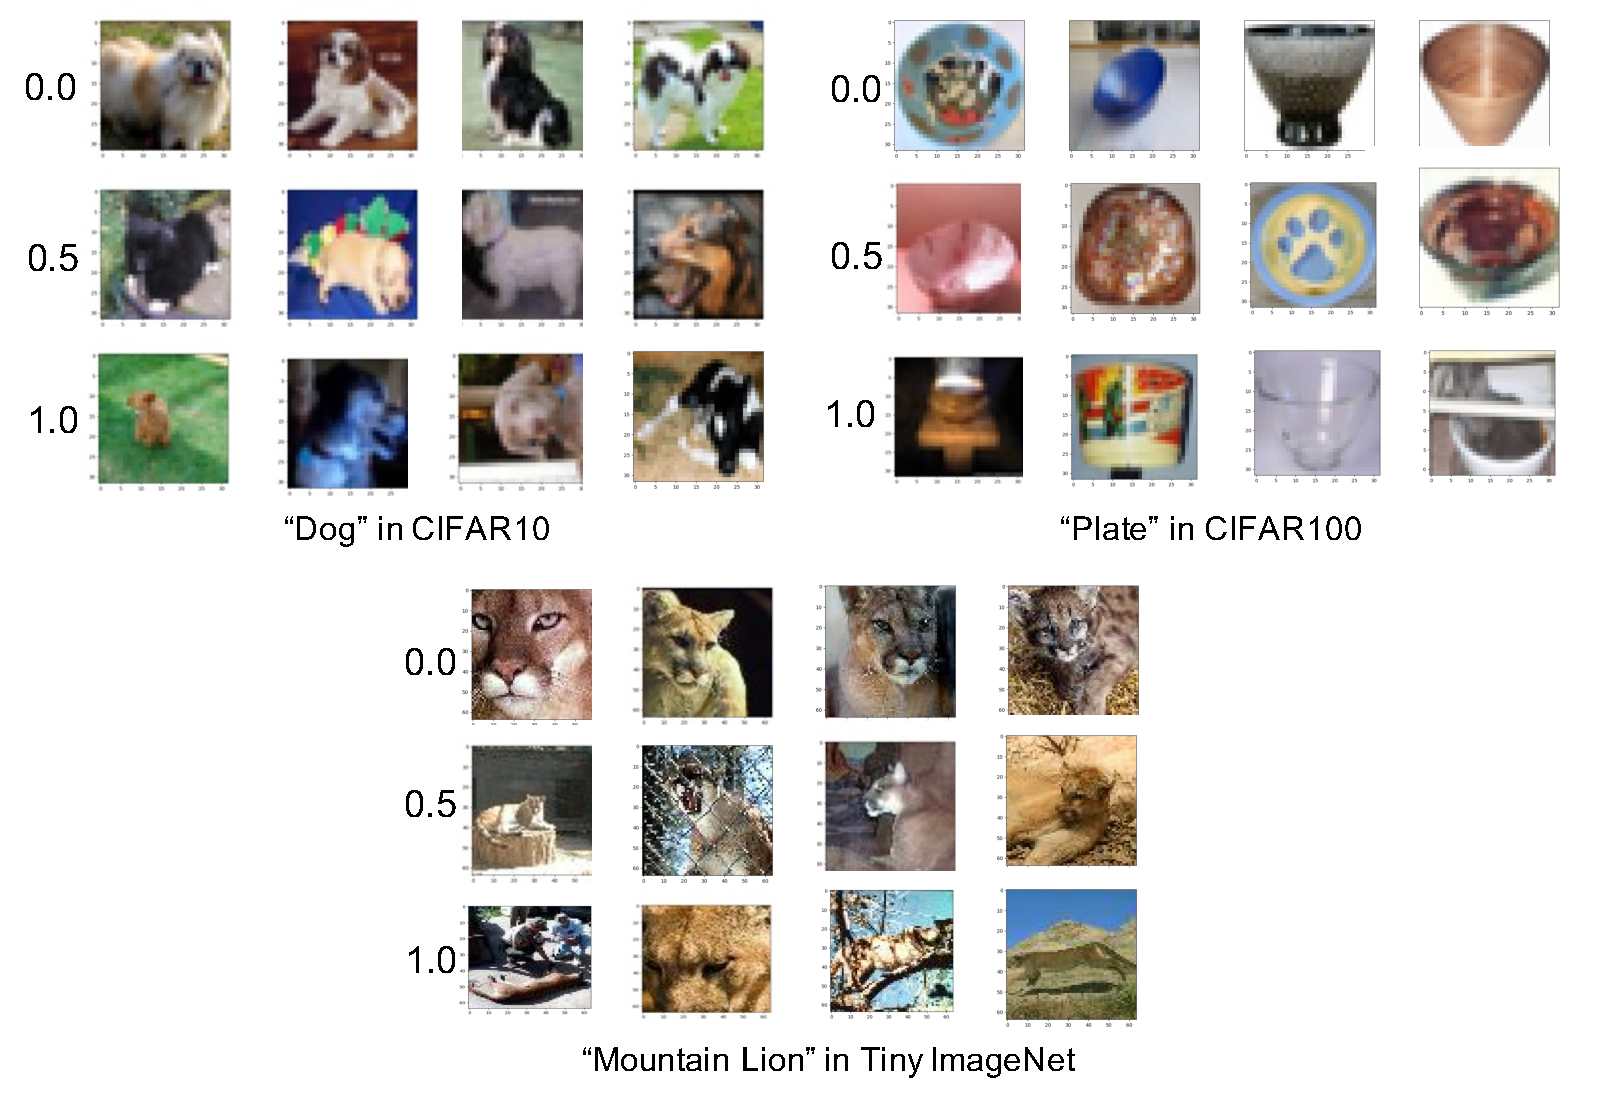
\includegraphics[width = 0.9\linewidth]{figures/atypical_examples.pdf}
    \caption{Examples of Images with Different Memorization Values}
    \label{fig:show_mem}
\end{figure}

\newpage
In Fig.~\ref{fig:hist}, we provide histograms to show the distribution of the estimated memorization values of all training samples from CIFAR10, CIFAR100 and Tiny~ImageNet. From Fig.~\ref{fig:hist}, we can observe that atypical samples (with high memorization value > 0.15) consist of a significant fraction (over 40\% \& 50\% respectively) in CIFAR100 and Tiny~ImageNet. In CIFAR10, they also consist of a non-ignorable fraction which is over 10\%.
\begin{figure}[h]
\centering
\subfloat[CIFAR100.]{
\begin{minipage}[c]{0.3\textwidth}
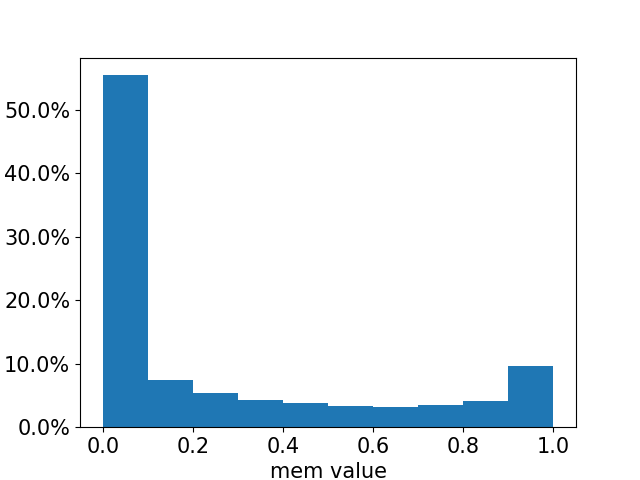
\includegraphics[width = 1.0\textwidth]{figures/hist_cifar100.png}
\end{minipage}
}
\hspace*{0.0cm}
\subfloat[CIFAR10.]{
\begin{minipage}[c]{0.3\textwidth}
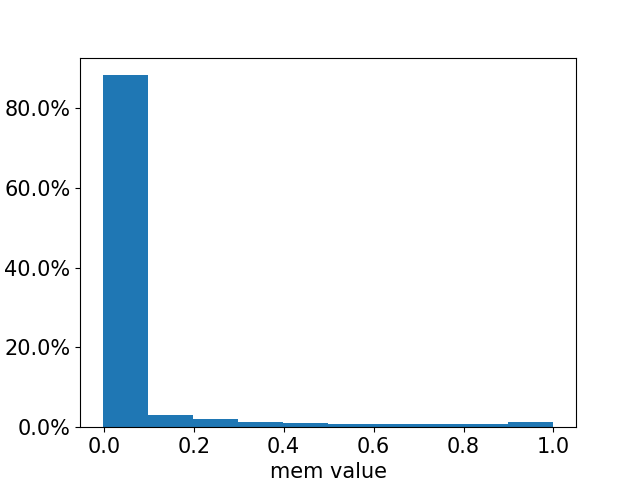
\includegraphics[width = 1.0\textwidth]{figures/hist_cifar10.png}%
\end{minipage}
}
\hspace*{0.0cm}
\subfloat[Tiny~ImageNet.]{
\begin{minipage}[c]{0.3\textwidth}
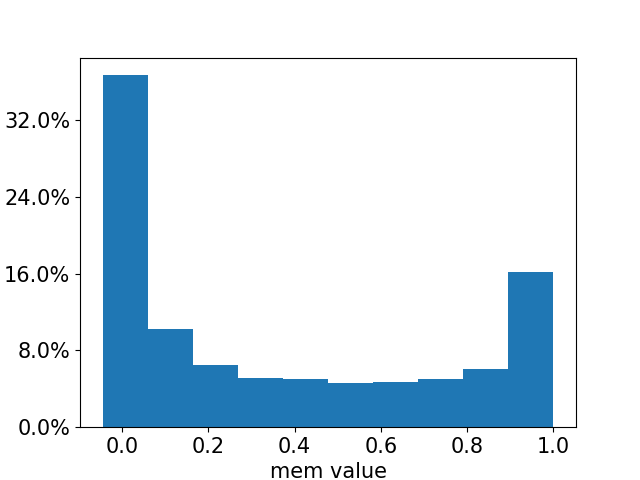
\includegraphics[width = 1.0\textwidth]{figures/hist_imagenet.png}%
\end{minipage}
}
\caption{Frequencies of Training samples with Different \textbf{Memorization Values} in Various Datasets}
\label{fig:hist}
\end{figure}


In Fig.~\ref{fig:show_pair}, we provide several pairs of images with high influence value (as defined in Section~\ref{sec:def_atypical}) which is over 0.15. In each pair, the training sample also has a high memorization value over 0.15. These examples suggest that there exist atypical samples in both training \& test sets of CIFAR10, CIFAR100 and Tiny~ImageNet. A pair of atypical samples (in the training set and test set) with a high influence value are visually very similar. Moreover, since they have high influence values, removing the atypical samples in the training set is very likely to cause the model to fail on the test atypical samples. Therefore, without memorizing the atypical sample in the training set, the model can hardly predict the atypical samples in the test set.
\begin{figure}[h]
    \centering
    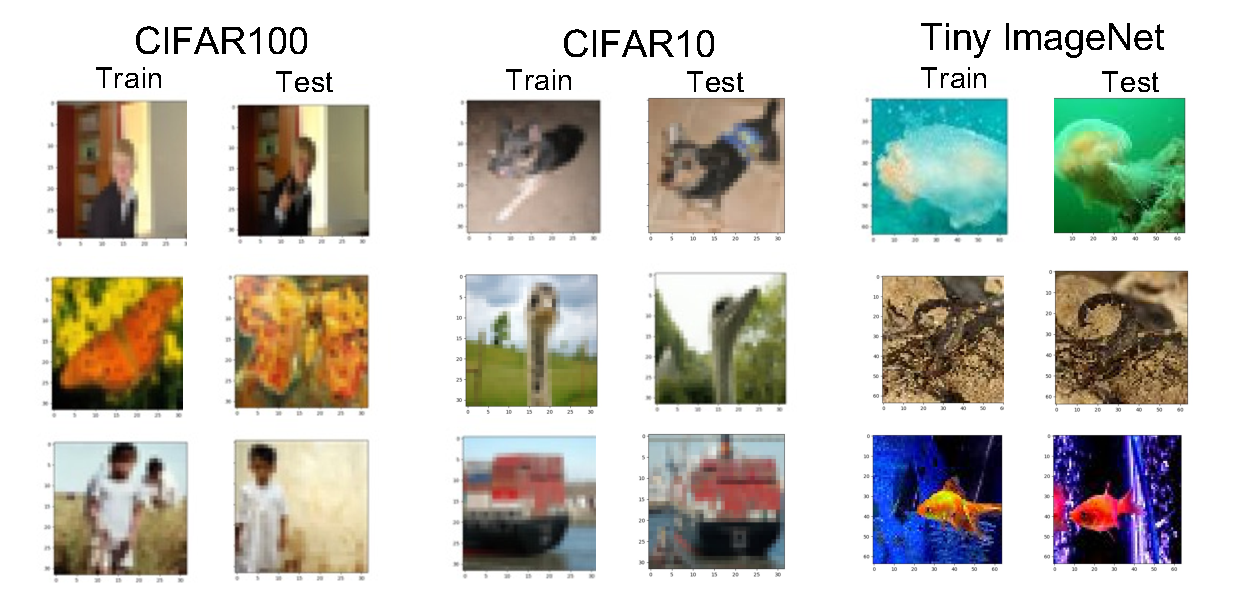
\includegraphics[width = 0.75\linewidth]{figures/pair.pdf}
    \caption{High Influence Pairs with Influence Value > 0.15}
    \label{fig:show_pair}
\end{figure}




